% Chapter 11 -- Symbolic Programming

\chapter{Symbolic Programming}
\TallC{All} symbolic programming is based on \textbf{rules} --- a set of generalized instructions that tells the computer how to transform one set of \textbf{tokens} into another. An assembler, \textit{e.g.}, inputs a series of machine instructions in mnemonic form and outputs a series of numbers that represent the actual machine instructions in executable form. A FORTH compiler translates a definition into a series of addresses of previously defined objects. Even higher on the scale of complexity, a FORTRAN compiler inputs high-level language constructs formed according to a certain \textbf{grammar} and outputs an executable program in another language such as assembler, machine code or C.

What do rules have to do with scientific problem-solving? The crucial element in the rule-based style of programming is the ability to specify general \textbf{patterns} or even classes of patterns so the computer can recognize them in the input and take appropriate action.

For example, in a modern high-energy physics experiment the rate at which events (data) impinge on detectors might be $10^{7}$ discrete events per second. Since each event might be represented by 5-10 numbers, the storage requirements for recording the results of a search for some rare process, lasting 3-6 months of running time, might be $10^16$ bytes, or $10^7$ high-capacity disk drives! Clearly, so much storage is out of the question and most of the incoming data must be discarded. That is, such experiments demand extremely fast filtering methods that can determine - in 10-20$\mu$sec - whether a given event is interesting. The criteria for "interesting" may be quite general and may need to be changed during the running of the experiment. In a word, they must be specified by some form of pattern recognition program rather than hard-wired.

Another area where pattern recognition helps the scientist is computer algebra. Closely related is the ability to translate mathematical formulae into machine code. So far we have stressed a FORTH programming style natural to that language, namely postfix notation, augmenting it primarily for readability or abstracting power. It cannot be denied, however, that sometimes it is useful simply to be able to write down a mathematical formula and have it translated automatically into executable form. This chapter develops the tools for symbolic programming and illustrates their use with a typical algebra program and a simple FORmula TRANslator.

\section{Rules}
Before we can specify rules we need a language to express them in. We need to be able to describe the \textbf{grammar} of the rules in some way. The standard notation states rules as \textbf{regular expressions\sepfootnote{11_01}}. The following rules describing some parts of FORTRAN illustrate how this works.

\begin{verbatim}
\ Rules for FORTRAN

\ NOTATION:
\ |         -> "or"
\ ^         -> "unlimited repetitions"
\ ^n        -> "0-n repetitions"
\ Q         -> "empty set"
\ &         -> + | -
\ %         -> * | /
\ <d>       -> "digit"

\ NUMBERS:
\ <int>     -> {-|Q} {<d> <d> ^8}
\ <exp't>   -> {dDeE} {&|Q}{<d> <d> ^2} | Q
\ <fp\#>    -> {-|Q}{ <d> | Q} . <d> ^ <exp't>

\ FORMULAS:
\ <assign>  -> <subj> = <expression>
\ <id>      -> <letter> {<letter>|<d>}^6
\ <subject> -> <id> {<idlist> | Q}
\ <idlist>  -> ( <id> {, <id> } ^)
\ <arglist> -> ( <expr'n> {, <expr'n>}^)
\ <func>    -> <id> <arglist>
\ <expr'n>  -> <terrn> | <terrn> & <expr'n>
\ <terrn>   -> <fctr> | <fctr> % <trm> | <fctr>**<fctr>
\ <factor>  -> <id> | <tp#> |(<expr'n> )| (tum)

\end{verbatim}

We use angular brackets "<", ">" to set off "parts of speech" being defined, and arrows "->" to denote "is defined by". Other notational conventions, such as "|" to stand for "or", are listed in the "NOTATION" section of the rules list, mainly for mnemonic reasons. A statement such as

\begin{verbatim}
\ <int>     -> {-|Q}<d><d>^8
\end{verbatim}

therefore means "an integer is defined by an optional leading minus sign, followed by 1 digit which is in turn followed by as many as 8 more digits". Similarly, the phrase

\begin{verbatim}
\ <assign>  -> <subj> = <expression>
\end{verbatim}

means “an assignment statement consists of a subject --a symbol that can be translated into an address in memory-- followed by an equals sign, followed by an expression". Literal symbols -- parentheses, decimal points, commas-- are shown in \textbf{bold} type.

Note that some of these definitions are \textbf{recursive}. A statement such as

\begin{verbatim}
\ <expr'n>  -> <term> | <term> & <expr'n>
\end{verbatim}

seems to be defined in terms of itself. So it is a good bet the program that recognizes and translates a FORTRAN expression will be recursive, even if not explicitly so.

\section{Tools}
\TallC{In} order to apply a rule stated as a regular expression, we need to be able to recognize a given pattern. That is, given a string, we need -say- to be able to state whether it is a foating point number or something else. We want to step through the string, one character at a time, following the rule

\begin{verbatim}
\ <fp#>     -> {-|Q}{{d . | .d | d} d ^ exp't
\end{verbatim}

This pattern begins with a minus or nothing, followed by a digit and a decimal point or a decimal point and a digit or a digit with no decimal point, followed by zero or more digits, then an exponent.

\subsection{Pattern recognizers}
\TallC{One} often sees pattern recognizers expressed as complex logic trees, \textit{i.e.} as sequences of nested conditionals, as in Fig. \ref{fig:11_01} on page \pageref{fig:11_01} below. As we see, the tree is already five levels deep, even though we have concealed the decisions pertaining to the exponent part of the number in a word \textbf{exponent?}. When programmed in the standard procedural fashion with \bc{IF...ELSE...THEN} statements, the program becomes too long

\begin{figure}[H]
\centering
\begin{tikzpicture}[framed, every edge/.style  = {draw,-{Kite[length=6pt,width=4pt]}, line width=0.5mm}]
    % Start
    \node[inner sep=0pt, anchor=center] (start) at (0,0) {};
    
    % 1st Branch Nodes
    \node[coordinate,below      =1.75cm of start]               (1branch)   {};
    \node[coordinate,below  left=0.5cm and 0.5cm of 1branch]    (1n)        {};
    \node[coordinate,below      =0.75cm of 1n]                  (11n)       {};
    \node[coordinate,below right=1.5cm and 1.5cm of 1branch]    (1y)        {};
    \node[inner sep=0pt, anchor=north] (1yotimes) at (1y) {\LARGE $\otimes$};
    
    % 2nd Branch Nodes
    \node[coordinate,below      =0.75cm of 1yotimes]            (2branch)   {};
    \node[coordinate,below right=1.5cm and 1.5cm of 2branch]    (2n)        {};
    \node[coordinate,below      =1.0cm of 2branch]              (2y)        {};
    
    % 3rd Branch Nodes
    \node[coordinate,below=0.75cm of 2n]                        (3branch)   {};
    \node[coordinate,below  left=1.0cm and 1.5cm of 3branch]    (3n)        {};
    \node[coordinate,below right=1.0cm and 1.5cm of 3branch]    (3y)        {};
    \node[inner sep=0pt, anchor=north] (3yotimes) at (3y) {\LARGE $\otimes$};
    
    % 4th ***left*** Branch Nodes
    \node[coordinate,below=0.75cm of 3n]                        (l4branch)  {};
    \node[coordinate,below=0.75cm of l4branch]                  (l4n)       {};
    \node[coordinate,below  left=1.5cm and 2.0cm of l4branch]   (l4y)       {};
    \node[coordinate,below=0.5cm of l4y]                        (l44y)      {};

    % 4th ***right*** Branch Nodes
    \node[coordinate,below=0.5cm of 3yotimes]                   (r4branch)  {};
    \node[coordinate,below right=1.25cm and 1.0cm of r4branch]  (r4n)       {};
    \node[coordinate,below=1.0cm of r4branch]                   (r4y)       {};
    
    % 5th Branch Nodes
    \node[coordinate,below=0.75cm of r4n]                       (5branch)   {};
    \node[coordinate,below=0.75cm of 5branch]                   (5n)        {};
    \node[coordinate,below right=1.0cm and 1.5cm of 5branch]    (5y)        {};
    \node[coordinate,below=0.75cm of 5y]                        (55y)       {};
    
    % Start
    \draw (start)       edge                                (1branch)   ;
    
    % 1st Branch edges
    \draw (1branch)     edge  node[xshift=-0.5cm] {No}      (1n)        ;
    \draw (1n)          edge                                (11n)       ;
    \draw (1branch)     edge  node[xshift=0.4cm]  {Yes}     (1y)        ;
    
    % 2nd Branch edges
    \draw (1yotimes)        edge                            (2branch)   ;
    \draw (2branch)     edge  node[xshift=0.4cm]  {No}      (2n)        ;
    \draw (2branch)     edge  node[xshift=-0.4cm] {Yes}     (2y)        ;
    
    % 3rd Branch edges
    \draw (2n)          edge                                (3branch)   ;
    \draw (3branch)     edge  node[xshift=-0.5cm] {No}      (3n)        ;
    \draw (3branch)     edge  node[xshift=0.5cm]  {Yes}     (3y)        ;
    
    % 4th ***left*** Branch edges
    \draw (3n)          edge                                (l4branch)  ;
    \draw (l4branch)    edge  node[xshift=0.4cm]  {No}      (l4n)       ;
    \draw (l4branch)    edge  node[xshift=-0.6cm] {Yes}     (l4y)       ;
    \draw (l4y)         edge                                (l44y)      ;
    
    % 4th ***right*** Branch edges
    \draw (3yotimes)    edge                                (r4branch)  ;
    \draw (r4branch)    edge  node[xshift=0.4cm]  {No}      (r4n)       ;
    \draw (r4branch)    edge  node[xshift=-0.4cm] {Yes}     (r4y)       ;
    
    % 5th Branch edges
    \draw (r4n)         edge                                (5branch)   ;
    \draw (5branch)     edge  node[xshift=-0.4cm] {No}      (5n)        ;
    \draw (5branch)     edge  node[xshift=0.5cm]  {Yes}     (5y)        ;
    \draw (5y)          edge                                (55y)       ;
    
    % All repeats
    \node[circle, fill=black, draw, below=0.0cm of 2y]  (2yrepeat)  {};
    \node[circle, fill=black, draw, below=0.0cm of r4y] (r4yrepeat) {};
    
    % All Exits
    \node[rectangle, draw, minimum width=0.5cm, minimum height=0.5cm, pattern=dots, below=0.0cm of 11n  ] (11nexit) {};
    \node[rectangle, draw, minimum width=0.5cm, minimum height=0.5cm, pattern=dots, below=0.0cm of l44y ] (l44yexit){};
    \node[rectangle, draw, minimum width=0.5cm, minimum height=0.5cm, pattern=dots, below=0.0cm of l4n  ] (l4nexit) {};
    \node[rectangle, draw, minimum width=0.5cm, minimum height=0.5cm, pattern=dots, below=0.0cm of 5n   ] (5nexit)  {};
    \node[rectangle, draw, minimum width=0.5cm, minimum height=0.5cm, pattern=dots, below=0.0cm of 55y  ] (55yexit) {};
    
    % All Text
    \node[below right=0.0cm and 0.1cm of start, align=left] (starting)  {START\\Get first char\\"-" or digit?};
    \node[align=left, below=0.0cm of 11nexit, ] (11nef)  {Exit,\\return\\"false"};
    \node[align=left, below=0.0cm of l44yexit,] (l44yet) {Exit,\\return\\"true"};
    \node[align=left, below=0.0cm of l4nexit, ] (l4nef)  {Exit,\\return\\"false"};
    \node[align=left, below=0.0cm of 5nexit,  ] (5nef)   {Exit,\\return\\"false"};
    \node[align=left, below=0.0cm of 55yexit, ] (55yet)  {Exit,\\return\\"true"};
    
    % All boardered rectangles
    \node[rectangle, draw=black, below   left=0.0cm and 0.2cm of 1y]  (1ybegin)      {begin};
    \node[rectangle, draw=black, below   left=0.0cm and 0.2cm of 2y]  (2ybrepeat)    {repeat};
    \node[rectangle, draw=black, below  right=0.0cm and 0.2cm of 2n]  (2nbdecimal)   {decimal point};
    \node[rectangle, draw=black, below   left=0.0cm and 0.2cm of 3y]  (3ybegin)      {begin};
    \node[rectangle, draw=black, below   left=0.0cm and 0.2cm of 3n]  (3nbexponent)  {exponent?};
    \node[rectangle, draw=black, below   left=0.0cm and 0.2cm of r4y] (r4ybrepeat)   {repeat};
    \node[rectangle, draw=black, below  right=0.0cm and 0.2cm of r4n] (r4nbexponent) {exponent?};
    
\end{tikzpicture}
\caption{\textit{Logic tree for <floating point \#>}} \label{fig:11_01}
\end{figure}

and too complex either for easy comprehension or for easy maintainance\sepfootnote{11_02}.

It has been known for many years that a better way to apply general rules - \textit{e.g.}, to detemiine whether a given string conforms to the rules for "foating point number" --- uses \textbf{finite state machines} (FSMs -we define them in \ref{chap:11_02_02} below). Here is an example, written in standard FORTH:

\begin{lstlisting}
    \ determine whether the string at Sadr is a fp#
    :skip-   ( adr -- adr' ) DUP C@ ASCII - = - ;
    :skip_dp ( adr -- adr' ) DUP C@ ASCII . = - ;
    \ NOTE: these "hacks" assume "true" = -1.
    :digit?  ( char -- f ) ASCII 9 ASCII 0 WITHIN ;
    : skip_dig ( adr2 adr1 -- adr2 adr1')
        BEGIN   DDUP > OVER C@ digit? AND
        WHILE     1+  REPEAT ;   \... cont'd below
    :dDeE?   ( char -- f) 95 AND \->uppercase
        DUP ASCII D = SWAP ASCII E = OR ;

    : skip_exponent ... ; \ this definition shown below

    :fp#?    ( $adr -- f )
        DUP 0 OVER COUNT + C! \ add terminator
        DUP C@ 1+ OVER C!     \ count = count+1
        COUNT OVER + 1- SWAP  ( -- $end $beg )
        skip- skip_dig skip_dp skip_dig
        skip_exponent
        UNDER =          \ $beg' = $end?
        SWAP C@ 0= AND ; \ char[$beg']=terminal?
\end{lstlisting}

The program works like this:

\begin{itemize}
    \item Append a unique terminal character to the string.
    \item If the first character is "-" advance the pointer 1 byte, otherwise advance 0 bytes.
    \item Skip over any digits until a non-digit is found.
    \item If that character is a decimal point skip over it.
    \item Skip any digits following the decimal point.
    \item A foating point number terminates with an exponent formed according to the appropriate rule (p. 261). \bc{skip_exponent} advances the pointer through this (sub)string, or else halts at the first character that fails to fit the rule.
    \item Does the initial pointer (\$beg') now point to the calculated end of the string (\$end)? And is the last character ( char[\$beg'] ) the unique terminal? If so, report "true", else report "false".
\end{itemize}

We deferred the definition of \bc{skip_exponent}. Using conditionals it could look like

\begin{lstlisting}
    : skip_exponent ( adr -- adr' )
        DUP C@ dDeE?    IF 1+ ELSE EXIT THEN
        skip- skip+
        DUP C@ digit?   IF 1+ ELSE EXIT THEN
        DUP C@ digit?   IF 1+ ELSE EXIT THEN
        DUP C@ digit?   IF 1+ ELSE EXIT THEN ;
\end{lstlisting}

which,as we see in Fig. \ref{fig:11_02} below, has nearly as convoluted a logic tree as Fig. \ref{fig:11_01} on page \pageref{fig:11_01} above.

\subsection{finite state machines}\label{chap:11_02_02}

\TallC{Just} as we needed a FSM to achieve a graceful definition of \bc{fp\#?}, we might try to define \bc{skip_exponent} as a state machine also. This means it is time to define what we mean by finite state machines. (We restrict attention to \textbf{deterministic} FSMs.) A \textbf{finite state machine\sepfootnote{11_03}\sepfootnote{11_04}} is a program (originally it was a hard-wired switching circuit\sepfootnote{11_05}) that takes a set of discrete, mutually exclusive

\begin{figure}[H]
\centering
\begin{tikzpicture}[framed, every edge/.style  = {draw,-{Kite[length=6pt,width=4pt]}, line width=0.5mm}]
    % Start
    \node[inner sep=0pt, anchor=center] (start) at (0,0) {};
    
    % 1st Branch Nodes - first split
    \node[coordinate,below      =1.0cm of start]                (1branch)   {};
    \node[coordinate,below right=1.0cm and 1.0cm of 1branch]    (1n)        {};
    \node[coordinate,below      =0.5cm           of 1n]         (11n)       {};
    \node[coordinate,below  left=0.0cm  and 1.5cm of 1branch]   (1y)        {};
    \node[coordinate,below  left=0.75cm and 0.0cm of 1y]        (11y)       {};
    \node[coordinate,below  left=0.75cm and 0.0cm of 11y]       (111y)      {};
    
    % 2nd Branch Nodes - after skip+
    \node[coordinate,below  left=0.75cm and 0.0cm of 111y]      (2branch)   {};
    \node[coordinate,below right=1.0cm and 1.0cm of 2branch]    (2n)        {};
    \node[coordinate,below      =0.5cm           of 2n]         (22n)       {};
    \node[coordinate,below  left=0.0cm and 1.5cm of 2branch]    (2y)        {};
    
    % 3rd Branch Nodes - 
    \node[coordinate,below  left=0.75cm and 0.0cm of 2y]        (3branch)   {};
    \node[coordinate,below right=3.0cm and 0.0cm of 3branch]    (3n)        {};
    \node[coordinate,below  left=0.75cm and 0.75cm of 3branch]  (3y)        {};
    \node[coordinate,below  left=0.75cm and 0.0cm of 3y]        (33y)       {};
    \node[coordinate,below right=0.75cm and 0.75cm of 33y]      (333y)      {};
    
    % 4th Branch Nodes
    \node[coordinate,below right=3.0cm and 0.0cm of 3n]         (4n)        {};
    \node[coordinate,below  left=0.75cm and 0.75cm of 3n]       (4y)        {};
    \node[coordinate,below  left=0.75cm and 0.0cm of 4y]        (44y)       {};
    \node[coordinate,below right=0.75cm and 0.75cm of 44y]      (444y)      {};
    
    % Start
    \draw (start)       edge                                (1branch)   ;
    
    % 1st Branch edges
    \draw (1branch)     edge  node[xshift=0.5cm]    {No}    (1n)    ;
    \draw (1n)          edge                                (11n)   ;
    \draw (1branch)     edge  node[yshift=0.2cm]    {Yes}   (1y)    ;
    \draw (1y)          edge                                (11y)   ;
    \draw (11y)         edge                                (111y)  ;
    
    % 2nd Branch edges
    \draw (111y)        edge                                (2branch)   ;
    \draw (2branch)     edge node[xshift=0.5cm]     {No}    (2n)        ;
    \draw (2n)          edge                                (22n)       ;
    \draw (2branch)     edge node[yshift=0.2cm]     {Yes}   (2y)        ;
    
    % 3rd Branch edges
    \draw (2y)          edge                                (3branch)   ;
    \draw (3branch)     edge node[xshift=0.5cm]     {No}    (3n)        ;
    \draw (3branch)     edge node[xshift=-0.3cm, yshift=0.3cm]      {Yes}   (3y)        ;
    \draw (3y)          edge                                (33y)       ;
    \draw (33y)         edge                                (333y)      ;
    
    % 4th Branch edges
    \draw (3n)          edge node[xshift=0.5cm]     {No}    (4n)        ;
    \draw (3n)          edge node[xshift=-0.3cm, yshift=0.3cm]      {Yes}   (4y)        ;
    \draw (4y)          edge                                (44y)       ;
    \draw (44y)         edge                                (444y)      ;
                                    
    % All Exits
    \node[rectangle, draw, minimum width=0.5cm, minimum height=0.5cm, pattern=dots, below=0.0cm of 11n ] (11nexit) {};
    \node[rectangle, draw, minimum width=0.5cm, minimum height=0.5cm, pattern=dots, below=0.0cm of 22n ] (22nexit) {};
    \node[rectangle, draw, minimum width=0.5cm, minimum height=0.5cm, pattern=dots, below=0.0cm of 4n  ] (4nexit)  {};
    
    % All Exit text
    \node[align=left, below right=0.0cm and 0.2cm of 11n] (11nE) {EXIT};
    \node[align=left, below right=0.0cm and 0.2cm of 22n] (22nE) {EXIT};
    \node[align=left, below right=0.0cm and 0.2cm of 4n]  (4nE)  {EXIT};
    
    % All other text
    \node[align=left, below right=0.0cm and 0.1cm of start]     (starting)  {eDeE?};
    \node[align=left, below  left=0.0cm and 0.1cm of 1y ]       (skipn)     {skip-};
    \node[align=left, below  left=0.0cm and 0.1cm of 11y]       (skipp)     {skip+};
    \node[align=left, below right=0.0cm and 0.1cm of 111y]      (1digit?)   {digit?};
    \node[align=left, above right=0.1cm and 0.1cm of 3branch]   (2digit?)   {digit?};
    \node[align=left, above right=0.1cm and 0.1cm of 3n]        (3digit?)   {digit?};
    \node[align=left, below  left=0.0cm and 0.1cm of 2y]        (1p)        {1+};
    \node[align=left, below  left=0.0cm and 0.1cm of 3y]        (2p)        {1+};
    \node[align=left, below  left=0.0cm and 0.1cm of 4y]        (3p)        {1+};
    
\end{tikzpicture}
\caption{\textit{Logic tree for <floating point \#>}} \label{fig:11_01}
\end{figure}

inputs and also maintains a \textbf{state variable} that tracks the history of the machine's inputs. According to which state the machine is in, a given input will produce different results. The FSM program is most easily expressed in tabular form, as in Table \ref{table:11_01}, which we interpret as follows:

\begin{itemize}
    \item each major column heading is an input.
    \item the inputs must be \textbf{mutually exclusive} and \textbf{exhaustive}; to exhaust all possibilities we include "other".
    \item each row represents the current state of the machine.
    \item each cell contains an action, followed by a state-transition.
\end{itemize}


\begin{table}[h!]
    \caption{Example of finite state machine arrow ( $\rightarrow$ ) means 'next state'}
    \begin{center}
        \begin{tabular}{|lllllllll|}
            \hline
\underline{Input:} & \underline{other} & & \underline{dDeE} & & \underline{+/-} & & \underline{digit} &    \\
        State      &     & $\rightarrow$ &    & $\rightarrow$ &   & $\rightarrow$ &        & $\rightarrow$ \\
      $\downarrow$ &                   & &                  & &                 & &                   &    \\
            0      & \lgray{Next}  & 5  & 1+           & 1  & \Aggray{Error}& 5   & \lgray{Next}  & 5      \\ &&&&&&&& \\
            1      & \lgray{Next}  & 5  & \lgray{Next} & 5  & 1+            & 2   & 1+    & 3              \\ &&&&&&&& \\
            2      & \lgray{Next}  & 5  & \lgray{Next} & 5  & \lgray{Next}  & 5   & 1+    & 3              \\ &&&&&&&& \\
            3      & \lgray{Next}  & 5  & \lgray{Next} & 5  & \lgray{Next}  & 5   & 1+    & 4              \\ &&&&&&&& \\
            4      & \lgray{Next}  & 5  & \lgray{Next} & 5  & \lgray{Next}  & 5   & 1+    & 5              \\ &&&&&&&& \\
            \hline
        \end{tabular}
    \end{center}
    \label{table:11_01}
\end{table}

\TallC{The} tabular representation of a FSM is much clearer than the logic diagram, Fig. \ref{fig:11_02}. Since the inputs must be \textbf{mutually exclusive}\sepfootnote{11_06} and \textbf{exhaustive}\sepfootnote{11_07}, there are \textit{never} conditions that cannot be fulfilled -that is, leading to "dead" code- as frequently happens with logic trees (owing to human frailty). This means the chance of introducing bugs is reduced by FSMs in tabular form.

FORTRAN, BASIC or Assembler can implement FSMs with computed GOTOs. In BASIC, \eg,

\begin{verbatim}
    DEF SUB FSM (c$, adress%)
    k% =0         ' convert input to column #
    C$=UCASE (c$)
    IF C$="D" OR C$="E" THEN k%=1
    IF C$="+" OR C$="-" THEN k%=2
    IF ASC(C$) >= 48 AND ASC(C$) <=57 THEN k%=3
    ' cont'd
\end{verbatim}


\begin{tabular}{ll}
\verb!      ' begin FSM proper!                                  & \\
\verb!    ON state\% *3 + k\% GOTO!                              & \\
\verb!      (0,1,2,3,4,5,6,7,8,9,10,11,12,13,14,15,16,17,18,19)! & \\
\verb!    0: state\%=5!               & \rdelim\}{4}{*}[' row 1]   \\
\verb!    1: adress\% = adress\% +1 : state\% = 1!               & \\
\verb!    2: CALL Error: state\% = 5!                            & \\
\verb!    3: state\%=5!                                          & \\
\verb!    4: state\%=5!               & \rdelim\}{4}{*}[' row 2]   \\
\verb!    5: state\%=5!                                          & \\
\verb!    6: adress\% = adress\% +1 : state\% = 2!               & \\
\verb!    7: adress\% = adress\% +1 : state\% = 3!               & \\
\verb!       ...... etc. ......!                                 & \\
\verb!    16:state\%=5!               & \rdelim\}{3}{*}[' row 4]   \\
\verb!    ...... etc.......!                                     & \\
\verb!    19:adress\% = adress\% +1 : state\% = 5!               & \\
\verb!    END SUB!                                               & 
\end{tabular}


The advantage of FSM construction using computed GOTOs is simplicity; its disadvantage is the linear format of the program that hides the structure represented by the state table, 11-1. CASE statements -as in C, Pascal or QuickBASIC- are no clearer. We can use a state table for documentation, but the subroutine takes more-or-less the above form.

\subsection{FSMs In FORTH}
\TallC{In} the preceding FORTH example we \textit{synthesized} the FSM from \bc{BEGIN} \bc{...} \bc{WHILE} \bc{...} \bc{REPEAT} loops. FORTH's lack of line-labels and GOTOs (jumps) imposed this method, producing code as untransparent as the BASIC version. The Eaker CASE statement can streamline the program,

\begin{lstlisting}
    CASE: ADVANCE? NEXT 1+ ;CASE
    : 1digit DUP C@ digit? ABS ADVANCE? ;
    : skip_exponent (adr -- adr')
        DUP C@ dDeE? IF 1+ ELSE EXIT THEN
        skip- skip+
        1digit 1digit 1digit ;
\end{lstlisting}

(three of four \bc{IF...ELSE...THEN}s have been factored out and disguised as \bc{CASE:} \bc{...} \bc{;CASE} ), but this does not much improve clarity. We still need the state transition table to understand the program.

Various authors have tried to improve FSMs in FORTH using what amount to line-labels and GOTOs\sepfootnote{11_08}\sepfootnote{11_09}\sepfootnote{11_10}. The resulting code is \textit{less} elegant than the BASIC version shown above.

\TallC{Whenever} we reach a dead end, it is helpful to return to the starting point, restate the problem and re-examine our basic assumptions One fact our preceding false starts make abundantly clear is that nowhere have we used the power of FORTH. Rather, our attempts merely imitated traditional languages in FORTH.

But FORTH is an endlessly protean language that lends itself to \textit{any} programming style. Ideally FORTH relies on names so cunningly chosen that programs become self-documenting-- readable at a glance.

Since state tables clearly document FSMs, it eventually occurred to me to let FORTH compile the state table --representing an FSM-- directly to that FSM!

\TallC{Compilation}implies a \textbf{compiling word}; after some experimentation\sepfootnote{11_11} I settled on the following usage\sepfootnote{11_12}:

\begin{figure}[H]
	\centering
    \begin{tabular}{|c|}
        \hline
        \begin{lstlisting}
    4 WIDE   FSM:   (exponents)
    \ Input: | other    | dDeE      | +/-       | digit  |
    \ state: - - - - - - - - - - - - - - - - - - - - - - -
     (0)     NEXT   >5    1+   >1   Error  >5   NEXT   >5
     (1)     NEXT   >5  NEXT   >5     1+   >2     1+   >3
     (2)     NEXT   >5  NEXT   >5   NEXT   >5     1+   >3
     (3)     NEXT   >5  NEXT   >5   NEXT   >5     1+   >4
     (4)     NEXT   >5  NEXT   >5   NEXT   >5     1+   >5 ;
        \end{lstlisting} \\
        \hline
    \end{tabular}
    \caption{Fig. 11-3 \textit{Form of a FORTH finite state machine}}
    \label{fig:11_03}
\end{figure}

The new defining word \bc{FSM:} has a colon ":" in its name remind us of its function. Its children clearly must "know" how many columns they have. The word \bc{WIDE} reminds us the newly created FSMs incorporate their own widths.

The column labels and table headers are merely commenst for following the state labels "$\textbackslash$" ; the state labels " \bc{( 0 )} ", " \bc{( 1 )} ", \etc are also comments, delineated with parentheses. Their only purpose is readability.

The actions -- \bc{NEXT, Error, 1+} -- in Fig. \ref{fig:11_03} are obvious: they; are simply previously-defined words. But what about the state: transitions " \bc{>1} ", " \bc{>2} ", ... ? The easiest, most mnemonic and natural way to handle state transitions defines them as \bc{CONSTANT}s

\begin{lstlisting}
    0 CONSTANT >0
    1 CONSTANT >1
    2 CONSTANT >2
      ... etc. ...
\end{lstlisting}

which are also actions to be compiled into the FSM. This follows the general FORTH principle that words should execute themselves\sepfootnote{11_13}.

\TallC{In} Chapter \ref{chap:05_02_06} we used components of the compiler, particularly the \bc{IMMEDIATE} word \bc{]} ("switch to compile mode"), to create self-acting jump tables. We apply the same method here: The defining word \bc{FSM:} will \bc{CREATE} a new dictionary entry, build in its width (number of columns) using " \bc{,} ", and then compile in the actions and state transitions as cfa’s of the appropriate words.

The runtime code installed by \bc{DOES>} provides a mechanism for finding the addresses of action and state transition corresponding to the appropriate input and current \textbf{state} (that is, in the cell of interest). Then the runtime code updates the \textbf{state}.

To allow* nesting of FSMs (\ie, compiling one into another), we incorporate the state variable for each child FSM within its data structure. This technique, using one extra memory cell per FSM, protects the \textbf{state} from accidental interactions, since if \textbf{state} has no name it cannot be invoked inadvertamly.

The FORTH code that does all this is
\begin{lstlisting}
    : WIDE 0 ;
    : FSM:      ( width 0 -- ) CREATE , , ]
        DOES>   ( col# -- )
            UNDER D@        ( -- adr col# width state )
            * + 1+ 4*       ( -- adr offset )
            OVER+           ( -- adr adr' )
            DUP@ SWAP 2+    ( -- adr [adr'] adr'+2 )
            ROT ! @EXECUTE   ;

    0 CONSTANT >0
    1 CONSTANT >1
    2 CONSTANT >2
    ... etc. ...
\end{lstlisting}

\TallC{We} are now in a position to use the code for \bc{(exponent)} (defined in Fig. \ref{fig:11_03} on page \pageref{fig:11_03} above) to define the key word \bc{skip_exponent} appearing in \bc{fp\#?}. The result is

\begin{lstlisting}
    : skip_exponent     ( adr -- adr' )
    ' (exponent) 0!     \ initialize state
    BEGIN   DUP C@ DUP  (  -- adr char )
        dDeE? ABS OVER  \ input -> col#
        +/-?    2 AND + SWAP
        digit?  3 AND + ( -- adr col# )
    ' (exponent) @      \ get state
    5 <                 \ not done?
    WHILE (exponent) REPEAT ;
\end{lstlisting}

\subsection{Automatic conversion tables}
\TallC{Our} preceding example used logic to \textbf{compute} (\textit{not} decide!) the conversion of input condition to a column number, \textit{via}

\begin{lstlisting}
    ( -- char) dDeE?  ABS OVER
               +/-?   2 AND + SWAP
               digit? 3 AND + ( -- col#)
\end{lstlisting}

When the input condition is a character, it is usually both faster and clearer to translate to a column number using a lookup table rather than tests and logic. That is, we can trade increased memory usage for speed. If a program needs many different pattern recognizers, it is worth generating their lookup tables via a defining word rather than crafting each by hand.

\begin{lstlisting}
    : TABLE:            ( -- #bytes )
        CREATE HERE     ( -- #bytes tab[0] )
        OVER ALLOT      \ allot #bytes in dictionary
        SWAP 0 FILL     \ initialize to all 0's
        DOES> + C@ ;   ( n tab[0] -- [tab[n]] )

    : install ( col# adr char.n char.1 -- ) \ fast fill
        SWAP 1+ SWAP
        DO DDUP I+ C! LOOP DDROP ;
\end{lstlisting}

Here is how we define a new lookup table:

\begin{lstlisting}
    128 TABLE: [exp]        \ define 128-byte table
    \ modify certain chars
    \ Note: all unmodified chars return col# 0

    1 ASCII d '[exp] + C!            \ col# 1
    1 ASCII D '[exp] + C!
    1 ASCII e '[exp] + C!
    1 ASCII E '[exp] + C!
    
    2 ASCII + '[exp] + C!            \ col# 2
    2 ASCII - '[exp] + C!

    3 '[exp] ASCII 9 ASCII 0 install \ col# 3
\end{lstlisting}

With the lookup table \bc{[exp]}, \bc{skip_exponent} becomes faster and more graceful,

\begin{lstlisting}
    : skip_exponent ( adr -- adr' )
        1 (exponent) 0!             \ state = 0
        BEGIN DUP C@                ( -- adr char )
            [exp]                   ( -- adr col# )
            ' (exponent) @          ( -- adr col# state )
            5 <                     \ not done?
        WHILE (exponent) REPEAT     ;
\end{lstlisting}

at a cost of 128 bytes of dictionary space. If dictionary space becomes tight, it would be perfeme simple to export the lookup tables to their own segment. in the same way we did with generic arrays in Chapter \ref{chap:05}.

\section{Computer algebra}
\TallC{One} of the most revolutionary recent developments in scientific  programming is the ability to do algebra on the computer. Programs like REDUCE, SCHOONSCIP, MACSYMA, DERIVE, and MATHEMATICA can automate tedious algebraic manipulations that might take hours or years by hand, in the process reducing the likelihood of error\sepfootnote{11_14}. The study of symbolic manipulation has led to rich new areas of pure mathematics\sepfootnote{11_15}. Here we illustrate our new tool (for compiling finite state automata) with a rule-based recursive program to solve a problem that does not need much formal mathematical background. The resulting program executes far more rapidly on a PC than REDUCE, \eg, on a large mainframe.

\subsection{Stating the problem}
\TallC{Dirac} $\gamma$-matrices are $4 \times 4$ traceless, complex matrices defined by a set of (anti)commutation relations\sepfootnote{11_16}. These are

\begin{equation} \label{eq:11_01}
\gamma^{\mu}\gamma^{v} + \gamma^{v}\gamma^{\mu} = 2 \eta^{\mu v}, \mu, v = 0,..., 3
\end{equation}

where $\eta^{\mu v}$ is a matrix-valued tensor,

\begin{equation}\label{eq:11_02}
    \eta^{\mu v} =
    \bordermatrix{
        \mu \textbackslash v & 0 &  1 &  2 &  3 \cr
        0 & I &  0 &  0 &  0 \cr
        1 & 0 & -I &  0 &  0 \cr
        2 & 0 &  0 & -I &  0 \cr
        3 & 0 &  0 &  0 & -I \cr
        }
\end{equation}

The \textbf{trace} of a matrix is defined to be the sum of its diagonal elements,

\begin{equation}\label{eq:11_03}
 Tr(\tr{A})\hat{=}\sum_{k=1}^{N}\tr{A}_{kk} .
\end{equation}

Clearly, traces obey the \textbf{distributive law}


\begin{subequations}\label{eq:11_04}
    \begin{equation}\label{eq:11_04_a}
        Tr(\tr{A} + \tr{B}) \equiv \Tr{A} + \Tr{B}
    \end{equation}
        as well as a kind of \textbf{commutative law},
    \begin{equation}\label{eq:11_04_b}
        Tr(\tr{A} \tr{B}) \equiv Tr(\tr{B} \tr{A}).
    \end{equation}
\end{subequations}

From Eq. \eqref{eq:11_01}, \eqref{eq:11_02}, and \eqref{eq:11_04_a},b we find

\begin{align}\label{eq:11_05}
    & Tr(\tr{A} \tr{B}) \equiv \frac{1}{2} \left[ Tr(\tr{A} \tr{B}) + Tr(\tr{B} \tr{A}) \right] = \frac{1}{2} Tr(\tr{A} \tr{B} + \tr{B} \tr{A}) \nonumber \\
    & = \frac{1}{2} 2 A \cdot B \Tr{I} \equiv 4 A \cdot B
\end{align}

where the ordinary vectors $A^{\mu}$ and $B^{v}$ form the (Lorentz-in-variant) "dot product"

\begin{equation}\label{eq:11_06}
A \cdot B \equiv A^{0} \cdot B^{0} - A^{1} \cdot B^{1} - A^{2} \cdot B^{2} - A^{3} \cdot B^{3}
\end{equation}

The trace of 4 gamma matrices can be obtained, analogous to Eq. \eqref{eq:11_05}, by repeated application of the algebraic laws 1-4:

\begin{align}\label{eq:11_07}
Tr(\tr{A}\tr{B}\tr{C}\tr{D}) & = 2A\cdot B Tr(\tr{C}\tr{D}) - Tr(\tr{B}\tr{A}\tr{C}\tr{D}) \nonumber \\
& \equiv 2 A\cdot B Tr(\tr{C}\tr{D}) - Tr(\tr{A}\tr{B}\tr{C}\tr{D}) \\
& \equiv 4 \left(A\cdot B C \cdot D - A\cdot C B\cdot D + A\cdot D B \cdot C \right) \nonumber 
\end{align}

We include Eq. \eqref{eq:11_07} for testing purposes. The factors of 4 in Eq. \eqref{eq:11_05} and \eqref{eq:11_07} do nothing useful, so we might as well suppress them in the, interest of a simpler program.

\subsection{The rules}
\TallC{We} apply formal rules analogous to those used in parsing a language\sepfootnote{11_17}. The rules for traces are:

\begin{verbatim}
\ Gemma Matrix Algebra Rules:

\ a              ->     string of booth <= 3
\ /              ->     delineator for factors
\ <factor>       ->     a/
\ product/       ->     e/b/c/d/
\ Tr( a/b/prod/) ->     a.b ( tr( prod/) ) - tr( a/prod/b'/ )
\ b'             ->     mark b as permuted
\ Tr( a/)        ->     0 ( a single factor is traceless)
\end{verbatim}

Repeated (adjacent) factors can be combined to produce a multiplicative constant:

\begin{align}\label{eq:11_08}
    \tr{B}\tr{B} \equiv B \cdot B ;
\end{align}

recognizing such factors can shorten the final expressions significantly, hence the rule

\begin{verbatim}
\ Tr( a/a/prod/) ->     a.a ( Tr( prod/) ).
\end{verbatim}

In the same category, when two vectors are orthogonal, $A\cdot B = 0$, another simplification occurs,

\begin{verbatim}
\ PERP A B       ->     A.B = 0.
\ Tr(A/B/prod/)  ->     -Tr( A/prod/B'/)
\end{verbatim}

The ability to recognize orthogonal vectors lets us (correctly)
include the trace of a product times the special matrix\sepfootnote{11_18}

\begin{equation}\label{eq:11_09}
    \gamma^{5} = i \gamma^{0} \gamma^{2} \gamma^{3} \gamma^{4} =
    \begin{pmatrix}
        0 &  0 &  1 &  0 \\
        0 &  0 &  0 &  1 \\
        1 &  0 &  0 &  0 \\
        0 &  1 &  0 &  0 
    \end{pmatrix}
\end{equation}

that anticommutes with all four of the $\gamma^{\mu}$:

\begin{equation}\label{eq:11_09}
    \gamma^{5}\gamma^{\mu} + \gamma^{\mu}\gamma^{5} = 0, \mu = 0,...,3 . \nonumber
\end{equation}

The fully antisymmetric tensor $\varepsilon_{v\mu\kappa\lambda} -\varepsilon_{v\mu\kappa\lambda}$, \etc, lets* us write

\begin{equation}\label{eq:11_10}
\gamma^{5}\tr{A}\tr{B}\tr{C} \equiv i \varepsilon_{v\mu\kappa\lambda} A^{\mu}B^{v}C^{\kappa}\gamma^{\lambda}, i = \sqrt{-1}  .
\end{equation}

A complete gamma matrix package includes rules for traces containing $\gamma^{5}$:

\begin{verbatim}
\ Trg5( a/b/c/d/x/) ->  i Tr( ^/d/x/)
\ ^.d               ->  [a,b,c,d] (antisymmetric product)
\ Note: ^.a = ^.b= ^.c = 0
\end{verbatim}

Since $\gamma$-matrices often appear in expressions like $(\tr{A} + m_{A}I)$, it will also be convenient to include the additional rules

\begin{Verbatim}[commandchars=\\\{\}]
\ *A/            ->     [A/ + m\textsubscript{A}]
\ Tr(*A/X/)      ->     m[A](Tr(x/) ) + Tr(x/ A/)
\end{Verbatim}

\subsection{The program}
\TallC{We} program from the bottom up, testing, adding, and modifying as we go. Begin with the user interface; we would like to say

\begin{lstlisting}
    TR( A/B/C/D/)
\end{lstlisting}

to obtain the output:

\begin{lstlisting}
    = A.BC.D-A.CB.D + A.DB.C ok
\end{lstlisting}

Evidently our program will input a string terminated by a right parenthesis "\bc{)}", \ie, the right parsnthesis tells it to stop inputting This can be done with the word\sepfootnote{11_19}

\begin{lstlisting}
    : get$ ASCII) TEXT PAD X$ $! ;
\end{lstlisting}

Since the rules are inherently recursive, we push the input string onto a stack before operations commence. What stack? Clearly we need a stack that can hold strings of “arbitrary” length. The strings cannot be too long because the number of terms of output, hence the operating time, grows with the number of factors N, in fact. like (gr: )1 .

\begin{figure}[H]
\centering
\begin{tikzpicture}[framed]
    % Nodes - prime path
    \node(start) at (0,0) {};
	\node[below=0.5cm of start] 	(1a) 		{};
	\node[ left=1.0cm of 1a]		(1decision) {};
	\node[below=0.5cm of 1decision]	(1skipn)	{};
	\node[below=0.5cm of 1skipn]	(1skipp) 	{};
	\node[below=1.0cm of 1skipp]	(2decision) {};
	\node[ left=1.0cm of 2decision]	(2a) 		{};
	
	\draw[-{Kite[length=6pt,width=4pt]}, line width=0.5mm] (start)     	-- (1a) 		;
    \draw[-{Kite[length=6pt,width=4pt]}, line width=0.5mm] (1a) 		-- (1decision) ;
    \draw[-{Kite[length=6pt,width=4pt]}, line width=0.5mm] (1decision) 	-- (1skipn)	;
    \draw[-{Kite[length=6pt,width=4pt]}, line width=0.5mm] (1skipn)	 	-- (1skipp) 	;
    \draw[-{Kite[length=6pt,width=4pt]}, line width=0.5mm] (1skipp) 	-- (2decision) ;
	\draw[-{Kite[length=6pt,width=4pt]}, line width=0.5mm] (2decision) 	-- (2a) 		;

\end{tikzpicture}
\caption{\textit{Logic tree for <exponent>}}\label{fig:11_01}
\end{figure}

Since the tokens are 1-byte integers smaller than 32, their 5th, 6th, and 7th bits can serve as flags to indicate their properties. For example, we need to indicate whether a factor was "starred", \ie. whether it represents $(\tr{A} + m_{A}I)$ or $\tr{A}$ , according to the rule

Since the rules are inherently recursive, we push the input string onto a \textbf{stack} before operations commence. What stack? Clearly we need a stack that can hold strings of "arbitrary" length. The strings cannot be \textit{too} long because the number of terms of output, hence the operating time, grows with the number of factors N, in fact, like $\left(\frac{1}{2}N)\right)$\bc{!}.

The pseudocode for the last word of the definition is clearly something like

\begin{lstlisting}
    : TR(   )get$   \ get a $ -terminated with ")"
            setup   \ push  $ on $stack
            parse ;
\end{lstlisting}

The real work is done by \bc{parse}, whose pseudocode is shown below in Fig. \ref{fig:11_04}; note how recursion simplifies the problem of matching left and right parentheses in the output.

Next we define the underlying data structures. Recursion demands a \textbf{stack} to hold strings in various stages of decomposition and permutation. Since the number of terms grows very rapidly with the number of factors, it will turn out that taking the trace of as many as 20 distinct factors is a matter of some weeks on -say- a 25 Mhz 80386 PC; that is, 14 or 16 factors are the largest practicable number. So if we make provision for expressions 20 factors long, that should be large enough for practical purposes\sepfootnote{11_20}.

\begin{figure}[H]
\centering
\begin{tikzpicture}[framed]
    % Nodes - prime path
    \node[inner sep=0pt, anchor=center] (start) at (0,0) {\LARGE $\otimes$};
    
    % Match code to start
    % Code on the right
    \node[right=1.0cm of start] (1a) {: parse\space\space\space\space\space \$pop};
    \node[below right=0.50cm and   0.5cm of 1a, anchor=text] at (1a.text) (2b)  {2factors (- - a b)};
    \node[below right=0.50cm and   0.0cm of 2b, anchor=text] at (2b.text) (3c)  {b=b'?};
    \node[below right=0.75cm and   0.0cm of 3c, anchor=text] at (3c.text) (4d)  {A.B};
    \node[below right=0.75cm and   0.0cm of 4d, anchor=text] at (4d.text) (5e)  {length(x) 0>};
    \node[below right=0.75cm and   0.0cm of 5e, anchor=text] at (5e.text) (6f)  {rearrange};
    \node[below right=0.50cm and   0.0cm of 6f, anchor=text] at (6f.text) (zz)  {};
    \node[below right=0.50cm and   0.0cm of zz, anchor=text] at (zz.text) (7g)  {." (" recurse :")"};
    \node[below right=1.00cm and   0.0cm of 7g, anchor=text] at (7g.text) (8h)  {recurse};
    \node[below right=1.00cm and  -0.5cm of 8h, anchor=text] at (8h.text) (9i)  {;};
    
    % Text on the right of code
    \node[right=4.2cm of start] (a1)    {\textbackslash{}  a/b/x/};
    \node[below right=0.5cm  and  0.0cm of a1, anchor=text] at (a1.text) (a2)   {\textbackslash{}  x/};
    \node[below right=0.5cm  and  0.0cm of a2, anchor=text] at (a2.text) (a3)   {\textbackslash{}  done?};
    \node[below right=0.75cm and  0.0cm of a3, anchor=text] at (a3.text) (a4)   {\textbackslash{}  output};
    \node[below right=0.75cm and  0.0cm of a4, anchor=text] at (a4.text) (a5)   {\textbackslash{}  more?};
    \node[below right=0.75cm and  0.0cm of a5, anchor=text] at (a5.text) (a6)   {\textbackslash{}  \~{}a/x/b'/};
    \node[below right=0.5cm  and  0.0cm of a6, anchor=text] at (a6.text) (xx)   {\textbackslash{}  x/};
    \node[below right=0.5cm  and  0.0cm of xx, anchor=text] at (xx.text) (a8)   {\textbackslash{}  Tr(x/};
    \node[below right=1.0cm  and  0.0cm of a8, anchor=text] at (a8.text) (a9)   {\textbackslash{}  Tr(\~a/x/b'/)};
    
    % Nodes - prime path
    \node[coordinate, below=0.75cm of start]    (yup)       {};
    \node[coordinate, below=2.25cm of start]    (nope)      {};
    \node[circle, fill=black, draw, below=3.875cm of start]                 (decision1) {};
    \node[circle, draw, fill=black, below=5.00cm of start, anchor=center]   (decision2) {};
    \node[rectangle, draw, below=5.75 of start, minimum width=1.5cm, minimum height=0.5cm, pattern=dots] (exit1) {};
    
    % Nodes - left path
    \node[coordinate,  left=1.5cm of yup]       (yup2)  	{};
    \node[coordinate,  left=1.5cm of nope]      (nope2)     {};
    \node[rectangle, draw, below=.5cm of nope2, minimum width=1.5cm, minimum height=0.5cm, pattern=dots] (exit2) {};

    % Connections - prime path
    \draw[-{Kite[length=6pt,width=4pt]}, line width=0.5mm] (start)     -- (yup) ;
    \draw[-{Kite[length=6pt,width=4pt]}, line width=0.5mm] (yup)       -- (nope) ;
    \draw[-{Kite[length=6pt,width=4pt]}, line width=0.5mm] (nope)      -- (decision1) ;
    \draw[-{Kite[length=6pt,width=4pt]}, line width=0.5mm] (decision1) -- (decision2) ;
    \draw[-{Kite[length=6pt,width=4pt]}, line width=0.5mm] (decision2) -- (exit1) ;
    
    % Connections - left path
    \draw[-{Kite[length=6pt,width=4pt]}, line width=0.5mm] (yup)     	--  (yup2) ;
    \draw[-{Kite[length=6pt,width=4pt]}, line width=0.5mm] (nope)    	--  (nope2) ;
    \draw[-{Kite[length=6pt,width=4pt]}, line width=0.5mm] (yup2)    	--  (exit2) ;

    % Labels
    \node[anchor=south west] at (yup2.north east)  {Yes};
    \node[anchor=south west] at (nope2.north east) {No};
    \node[below=0.01cm of exit1] {Exit};
    \node[below=0.01cm of exit2] {Exit};

\end{tikzpicture}
\caption{Pseudocode/flow diagram for "parse"} \label{fig:11_01_04}
\end{figure}

How deep an the \$stack get? The algorithm expressed by the rule

\begin{verbatim}
\ Tr( a/b/prod/) -> a.b ( Tr( prod/) ) - Tr( a/prod/b'/)
\end{verbatim}

suggests that for an expression of length n=2k, the maximum depth will be k + 1. Thus we should plan for a stack depth of at least 11, perhaps 12 for safety. Assuming factor-names up to three characters long, and strings of up to 20 names, we need $\approx$60 characters per string. My first impulse was to create a dynamic \textbf{\$stack} that could accomodate strings of variable length, meaning that some 330 bytes of storage would be needed, at the cost of some complexity in keeping track of the addresses. This is a big improvement on 720 bytes needed for a 60-wide fixed-width stack, of course. However, the convenience of a fixed-width \$stack led me ultimately to set up a table (array) of 20 names, whose indices would act as tokens; that is, the strings that actually go on the \$stack would be tokenized. The memory cost of the table together with a 12-deep, fixed-width \$stack is thus only 80 + 242 = 322 bytes.

\begin{lstlisting}
TASK GAMMA
\ FINITE STATE MACHINE
: WIDE 0 ;
: FSM: ( width 0 -- ) CREATE , , ]
    DOES> ( col# -- )
        UNDER D@        ( -- adr col# width state )
        * + 1+ 4*       ( -- adr offset )
        OVER +          ( -- adr adr1 )
        DUP@ SWAP 2+    ( -- adr [adr'] adr1+2 )
        EXECUTE@        ( -- adr [adr'] state' )
        ROT! EXECUTE    ;
0 CONSTANT >0 3 CONSTANT >3
1 CONSTANT >1 4 CONSTANT >4
2 CONSTANT >2 5 CONSTANT >5
\ END FINITE STATE MACHINE

\ Automatic conversion tables
: TAB:  ( #bytes -- )
    CREATE  HERE OVER ALLOT
            SWAP 0 FILL     \ init table
    DOES>   + C@ ;

: install   ( col# adr char.n char.1 -- )    \ fast fill
    SWAP 1+ SWAP
    DO DDUP I + C! LOOP DDROP ;
\ end automatic conversion tables

\ STRING HANDLING
HEX
\ Note: ?((( ...... ))) conditionally compiles "......"
FIND $! 0=
  ?((( : $! ( sadr dadr -- ) OVER C@ 1+  CMOVE ; )))
FIND $+ 0=
  ?((( : $+ ( adr$1 adr$2 -- pad )
    DUPC@   ( -- $adr a )
    >R 1+ OVER C@ PAD + 1+
    R@ <CMOVE PAD $!
    R> PAD C@ + 0 MAX FF MIN    PAD C! ; )))
DECIMAL
: 1+C!  ( adr -- ) DUPC@ '+ SWAP C! ;
: -BL  ( $adr -- )   \ delete all blanks from $
    DUP >R 0 PAD C! COUNT OVER + SWAP
    DO I C@ DUP@ 32 <>
        IF  PAD COUNT = C! PAD 1+C!
        ELSE DROP THEN
    LOOP    PAD R> $! ;
\ END STRING HANDLING

\ PARSE WORDS
\ Note: The factor *A/ in the input string
\ means (A/ + M sub A)
0 VAR star
: star! 123 IS star DROP ;  \ set 7th bit if 1st char=*

0 VAR #/                    \ counts # of factors
: +#/       AT #/ 1+!       DROP ; \ inc #/

: err CR -1 ABORT" Name-> letter (letter | numeral )*" ;
: +PAD ( char -- ) star OR       \ set bit 7
    PAD COUNT + C! PAD C@ '+ PAD C! 0 IS star ;
    
5 WIDE FSM: (factor)    (char col# -- )
\ input | other | letter | digit |   /   |   *   |
\ state -----------------------------------
(0)     err #0  +PAD >2  err  >0  +#/ >5  star! >1
(1)     err #0  +PAD >2  err  >1  +#/ >5  err   >1
(2)     err #0  +PAD >3  +PAD >3  +#/ >5  err   >2
(3)     err #0  +PAD >4  +PAD >4  +#/ >5  err   >3
(4)     err #0  DROP >4  DROP >4  +#/ >5  err   >4
    ;       \ terminate definition

128 TAB:    [factor]        \ convert char to col#
1 '[factor]     ASCII Z ASCII A install
1 '[factor]     ASCII z ASCII a install
2 '[factor]     ASCII 0 ASCII 9 install
3 '[factor]     ASCII / + C!
4 '[factor]     ASCII * + C!

: <factor>  (adr -- adr')
    PAD 0!  '(factor) 0! 0 IS star  \ initialize
    BEGIN DUPC@ DUP     [factor] (factor) 1+
        '(factor) @ 5 =
    UNTIL ;

CREATE factor{ 20 4* ALLOT OKLW     \ up to 20 factors
: } ( adr n - adr + 4*n) 4* + ; \ compute address

0 VAR N 0 VAR N1
CREATE  BUF$ 20 ALLOT OKLW      \ data structures

: unstar 127 AND ;  \ token[*A] = token[A] 128 OR
: $= ( $adr1 $adr2 -- f)
    -1 -ROT COUNT
    ROT COUNT ( -- $adr2+1 n2 $adr1+1 n1 )
    ROT DDUP =
    IF DROP
        0 DO  DUPC@ unstar  >R 1+
            OVER C@ unstar R>  <>
            IF ROT NOT -ROT LEAVE THEN
            SWAP 1+
        LOOP DDROP
    ELSE DDROP DDROP NOT THEN ;
: check.table ( -- )    \ prevent duplicate tokens
    -1 IS N1 LEAVE THEN
    LOOP ;

: +buf$ N N1 -1 = AND N1 -1 > N1 AND +
                                    \ token N or N1
    PAD 1+ C@ 128 AND OR            \ if star, set bit 7
    BUF$ DUPC@ + 1+ C! BUG$ 1+C! ;
                                    \ append token

: tokeniz ( $adr -- )                \ decompose into factors
    factor{ 80 0 FILL               \ initialize table
    COUNT OVER + ( -- $adr+1 $adr' ) \ addresses
    >R                  \ $adr' = $adr+LEN($) + 1
    0 BUF$ C!           \ init. buffer
    0 IS N              \ init. N
    BEGIN <factor>      \ begin loop; get factor
        check.table     \ prevent multiple entries
        +buf$           \ add factor to tokenized $
        N1 -1 =         \ not in table?
        IF PAD factor{ N } $!   \ put in table
            AT N 1+!    \ inc. N
        THEN
    DUP R@ = UNTIL      \ end loop
    DROP RDROP ;        \ clean up
\ END PARSE WORDS

\ $stack
CREATE $stack 20 20 * 2+ ALLOT OKLW     \ 2 for ptr
: $push ( $adr -- )
    DUPC@ 19 > ABORT" STRING TOO LONG!"
    $stack DUP@ DUP 19 > ABORT" $stack too deep!"
    20 * 2+ + $!    $stack 1+! ;
: $pop  ( $adr -- ) $stack DUP@ 1- 0 MAX
    DDUP SWAP !
    20 * 2+ + SWAP $!
\ end $stack

CREATE X$ 80 ALLOT OKLW \ buffer for input $, tail$
: get$ ASCII ) TEXT     \ input a $ terminated by )
    PAD -BL             \ delete blanks
    PAD X$ $! ;

: 1factor ( -- a )      \ get 1 factor, tail -> x$
    BUF$ 1+ C@          ( -- a )
    BUF$ COUNT 1- >R
    1+ X$ 1+ R@ <CMOVE  \ tail -> x$
    R> X$ C! ;          \ adjust count
: 2factors ( -- a b )   \ get 1st 2 factors
    1factor X$ BUF$ $! 1factor ;

0 VAR sign              \ emit correct sign
2 TAB: [sign]           \ make table
ASCII + '[sign]    C!   \ fill table
ASCII - '[sign] 1+ C!
: .sign ( a -- ) 64 AND 0> [sign] sign AND EMIT ;

\ Note: we mark prime (') by 64 OR (set bit 6 in token)
\   since 1st factor is never ', we set bit 6 for leading "-" sign
: prime!    64 OR  ;
: unprime   63 AND ;
: A.B   ( a b -- )      \ emit "dot product"
    unprime             \ b' -> b
    OVER .sign          \ emit sign
    SWAP unprime        \ drop leading "-"
    DDUP MAX -ROT MIN   \ sort factors
    factor{ SWAP } $.
    ASCII . EMIT factor{ SWAP } $.  -1 IS sign ;

: clean ( $adr -- )     \ unprime all factors
    COUNT OVER + SWAP
    DO I C@ unprime I C! LOOP ;


: rearrange      ( a b -- )
    1 BUF$  \ init buf$
    BUF$ X$ $+ PAD BUF$ $!       \ buf$-> _/x/
    prime!          ( -- a b' )
    BUF$ COUNT + C! BUF$ 1+C!    \ buf$-> _/x/b'/
    64 XOR       ( -- a xor 64 ) \ toggle sign of a
    BUF$ 1+ C! ; ( -- )          \ buf$-> ~a/x/b'/

: setup     X$ tokenize         \ form token$
            $stack 0!           \ init $stack
            0 IS sign           \ init sign flags
            BUF$ $push ;        \ input token$ on $ stack

\                               debugging code
: $$.   ( $adr -- ) COUNT OVER + SWAP   \ translate token$
    DUPC@ .sign factor{ OVER C@ unprime } $. ."/"
    1+ DO   factor{ I C@ unprime } $.
            I C@ 64 AND 0>              \ primed?
            IF ." '" THEN   ."/"
    LOOP ;
: dump$stack? DEBUG NOT IF EXIT THEN
    $stack 2+       ( -- $adr[0] )
    $stack @ DUP 0= \ $stack empty?
    IF DDROP CR ." $stack empty" EXIT THEN
    0 DO I 20 * OVER + CR $$. LOOP DROP ;
0 VAR DEBUG
: DEBUG-ON  -1 IS DEBUG ;
: DEBUG-OFF  0 IS DEBUG ;
\               end bebugging code

: (.    ."("  0 IS sign ;
: ).    .")" -1 IS sign ;
: parse dump$stack?
    BUF$    $pop    2factors ( -- a b )
    DUP     64 AND 0>        \ b = b'?
    IF      DDROP EXIT THEN
    DDUP A.B    ( -- a b )   \ output
    X$ C@ 0>                 \ more?
    IF  rearrange   \ buf$=    ~a/x/b'/
        BUF$ $push           \ ~a/x/b'/
        X$ clean X$ $push    \    x/
        (. RECURSE ).
           RECURSE
    ELSE    DDROP   THEN ;

: TR(   get$                 \ input $
        setup
        ." =" CR             \ for beauty
        parse ;
\end{lstlisting}

Since the tokens are 1-byte integers smaller than 32, their 5th, 6th, and 7th bits can serve as flags to indicate their properties. For example, we need to indicate whether a factor was "starred", \ie. whether it represents $(\tr{A} + m_{A}I)$ or $\tr{A}$ , according to the rule

\begin{verbatim}
\ *A/            ->     (A/ + m[A)).
\end{verbatim}

Again, we need to be able to indicate a "prime", showing that a factor has been permuted following the rule

\begin{verbatim}
\ Tr( a/b/prod/) ->     a.b ( tr( prod/) ) - tr( a/prod/b'/)
\end{verbatim}

Thus we set bit 7 (\bc{128 OR}) to indicate "star", and bit 6 (\bc{64 OR}) to indicate "prime".

We still need to indicate the leading sign. My first impulse was to use bit 5, but I realized the first factor is never permuted, hence, its 6th bit is available to signify the sign. It is toggled by the phrase \bc{64 XOR}. (In the \$stack pictures appearing in the Figures we indicate toggling by a leading "\bc{\~}".)

Programming these aspects is fairly trivial so we need not dwell on it. The entire program appears on pages 279 and 280 above.

Now we test the program:

\begin{lstlisting}
    TR( A/B/C/D/E/F/) =
    A.B(C.D(E.F)-C.E(D.F) + C.F(D.E))
   -A.C(D.E(B.F)-D.F(B.E) + B.D(E.F))
   +A.D(E.F(B.C)-B.E(C.F) + C.E(B.F))
   -A.E(B.F(C.D)-C.F(B.D) + D.F(B.C))
   +A.F(B.C(D.E)-B.D(C.E) + B.E(C.D)) ok
\end{lstlisting}

\TallC{Clearly} the concept works. Our next task is to incorporate branches to take care of "starred", as well as identical and/or orthogonal adjacent factors. The possible responses to the different cases are presented in decision-table form in Table \ref{table:11_02}:

To avoid excessively convoluted logic we eschew nested branching constructs. A finite state machine would be ideal for clarity; however, as Table \ref{table:11_02} makes clear, the logic is not really that of a FSM, besides which, the FSM compiler described above would

\begin{verbatim}

Input:    & a/b/x/   & *a/b/x/ & a/*b/x/ & a/a/x/ & a/b/x/,a.b=0

Resulting & ~a/x/b'/ & a/b/x/  & a/b/x/  & ...    & ...

$stack: XI b/XI a/x/ x/ "' a/x/b’l

Action(s): & a.b       & m[a]      & m[b]      & a.a       & RECURSE

           & (RECURSE) & (RECURSE) & (RECURSE) & (RECURSE) &

           & RECURSE   & RECURSE   & RECURSE

Note: characters shown in light typeface are \bc{EMIT}ed.
\end{verbatim}

have to be modified to keep its state variable on the stack, since otherwise it could not support recursion. The resulting pseudocode program is shown in Fig. \ref{fig:11_05}. Implementing the code is now straightforward, so we omit the details, such as how to define \bc{PERP} to appropriately mark the symbols. The simplest method is a linked list or table of some sort, that is filled by \bc{PERP} and consulted by the test word \bc{perps?}.


\TallC{How} might we implement a leading factor of $\gamma^{5}$? While there is no difficulty in taking traces of the form

\begin{equation}
Tr( \gamma^{5} \tr{A} \tr{B} \tr{C} \tr{D} ...) \equiv Tr(\varepsilon_{v\mu\kappa\lambda} A^{\mu} B^{v} C^{\kappa} \gamma^{\lambda} \tr{D} ...),
\end{equation}

\begin{figure}
    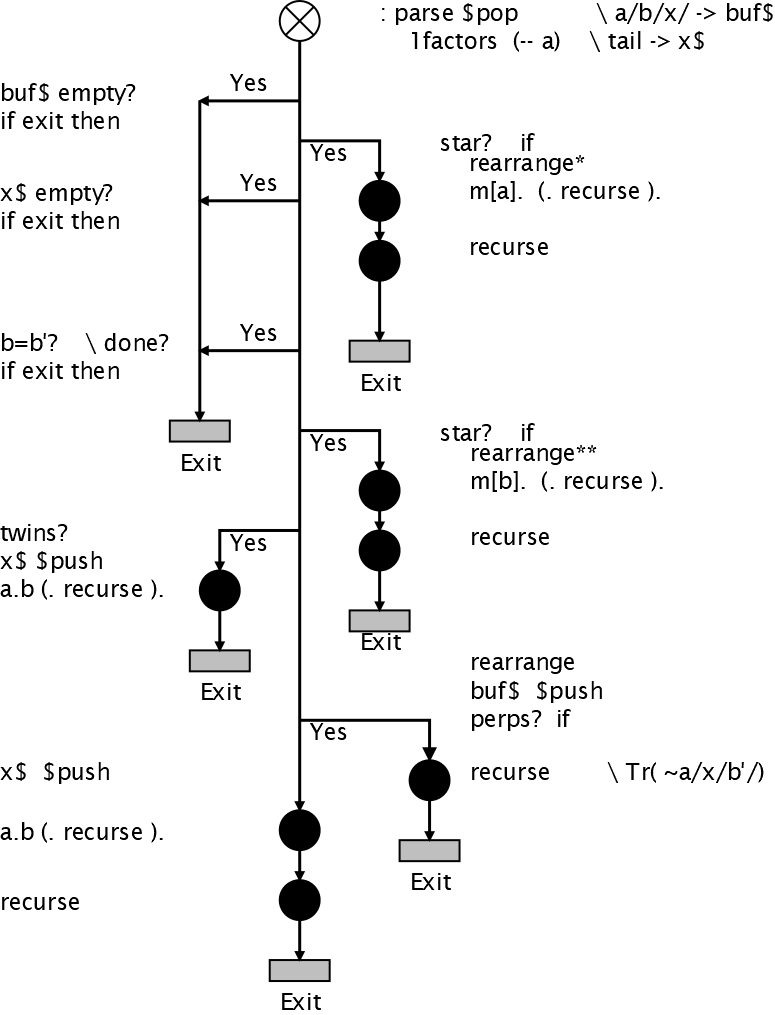
\includegraphics[width=\textwidth]{figure_11_5_diagram.png}
    \caption{Fig. 11-5 \textit{Pseudocode/flow diagram for extended "parse"}}
    \label{fig:11_05}
\end{figure}

so the key issue becomes decomposing leading starred factors, saving the pieces on the \$stack until at least three distinct unstarred factors are adjacent on the left. Replace these by a special 

expressions with $\gamma^{5}$ between "starred" factors are more difficult. However, the permutation properties of traces let us write, \eg,

\begin{align}
& Tr( (\tr{A} + m_{A})(\tr{B} + m_{B})\gamma^{5} \tr{C}(\tr{D} + m_{D})\tr{E} ... ) \\
\equiv & Tr(\gamma^{5}\tr{C}(\tr{D} + m_{D})\tr{E} ... (\tr{A} + m_{A})(\tr{B} + m_{B}) ,
\end{align}

so the key issue becomes decomposing leading starred factors, saving the pieces on the \$stack until at least three distinct unstarred factors are adjacent on the left. Replace these by a special 

token which stands for "\bc{^}" as shown on page \pageref{page:11_276}. This token is a marked orthogonal to all three of the vectors it represents, at the time it is inserted.

To avoid further extending \bc{parse}, probably the best scheme is to define a distinct word, \bc{Trg5(}, that uses the components of \bc{parse} to perform the above preliminary steps. Then \bc{Trg5(} will invoke \bc{parse} to do the rest of its work.

The only other significant task is to extend the output routine to

\begin{enumerate}
\item[a)] recognize the special "\bc{^}" token; and
\item[b)] replace dot products like "\bc{^.d}" by \bc{[a,b,c,d]}.
\end{enumerate}


\leftbar[1\linewidth]
A final remark: one or another form of vectoring can simplify \bc{parse} (relative to Fig. \ref{fig:11_05}) by hiding the recursion within words that execute the branches. We have avoided this method here because it conceals the algorithm, a distinct pedagogical disadvantage.
\endleftbar

\section{FORmula TRANslator}
\TallC{That} prehistoric language FORTRAN -despite its manifold deficiencies relative to FORTH - contains a useful and widely imitated invention that helps maintain its popularity despite competition from more modern languages: This is the FORmula TRANslator from which the name FORTRAN derives.

FORTH's lack of FORmula TRANslator is keenly felt. Years of scientific FORTH programming have not entirely eliminated my habit of first writing a pseudo-FORTRAN version of a new algorithm before reexpressing it in FORTH. Sometimes I will even write a test program in QuickBASIC$^{\copyright}$ before re-coding it in FORTH for speed and power, just to avoid worry about getting the arithmetic expressions correct.

\subsection{Rules of FORTRAN}
\TallC{A} FORmula TRANslator provides a nice illustration of rule-based programming. To maintain portability, we employ the standard FORTH kernel, omitting special HS/FORTH words as well as CODE words.

In principle we could provide a true compiler that translates formulae to machine code (or anyway, to assembler). But unless we use p-code or some such artifice\sepfootnote{11_21} we would lose all hope of portability. Thus, we take instead the simpler course of translating FORTRAN formulae to FORTH according to the rules

\begin{verbatim}
\ NUMBERS:
\ <int>          ->     {-| Q} {digit digit^8}
\ <exp't>        ->     {dDeE} {& | Q} {digit digit^2}| 0}
\ <fp#>          ->     {-| Q} {dig | Q} . dig^ <exp't>

\ FORMULAS:
\ <assignment>   ->     <subject> = <expression>
\ <id>           ->     letter {letter|digit}^6
\ <subject>      ->     <id>{<idlist> | Q}
\ <idlist>       ->     ( <id> {, <id> }^)
\ <arglist>      ->     ( <expr'n> {, <expr’n> }^)
\ <function>     ->     <id> <arglist>
\ <expression>   ->     <terrn> | < term> & <expr'n>
\ <term>         ->     <factor> | <factor> % <term>
\ <factor>       ->     <id> | <fp#> | ( <expr'n> ) |
                 ->     <factor> ** <factor>
\end{verbatim}

Clearly, the FORTH FORmula TRANslator could become the kernel of a more complete FORTRAN->FORTH filter by adding to the above rules for formulae the following rules for loops and conditionals:

\begin{verbatim}
\ DO LOOPS:
\ <label>        -> <integer>
\ <lim>          -> { <integer> | <id> }
\ <step>         -> {, <lim> | Q }
\ <do>           -> DO <label> <id> = <lim>, <lim> <step>

\ BRANCHING STRUCTURES:
\ <logical expr> -> <factor > .op. < factor >
\ <il0>          -> IF( <logical expr> ) <assignment>
\ <if1 >         -> IF( <logical expr> )THEN
\                       { <statement> }^
\                   END IF
\
\ <if2>          -> IF( <logical expr> )THEN
\                       { <statement> }^
\                   ELSE
\                       { <statement> }^
\                   END IF
\
\ <if3>          -> IF( <logical expr> )THEN
\                       { <statement> }^
\                   ELSEIF( <logical expr> )
\                       { <statement> }^
\                   END IF
\end{verbatim}

\subsection{Details of the Problem}
The general principles of compiler writing are of course well understood and have been described extensively elsewhere. Several computer science texts expound programs for formula evaluators\sepfootnote{11_22}. Once we have our translator, we can easily make it an evaluator by compiling the FORTH as a single word, then invoking it.

Let us proceed by translating a FORTRAN formula into FORTH code by hand. For simplicity, ignore integer arithmetic and assume all literals will be placed on the intelligent foating point stack (\textbf{ifstack}). Similarly assume all variable names in the program refer to \bc{SCALAR}s (see \ref{chap:05}). A word that has become fairly standard is \bc{\%}, which interprets a following number as floating point, and places it on the fstack. With these conventions, we see that we shall want to translate an expression like

\begin{lstlisting}
    A = -15.3E7*EXP(7/X) + Z/(W-SIN(THETA*PI/180/4)
\end{lstlisting}

into (generic) FORTH something like this:

\begin{lstlisting}
    % 4   REAL*8 >FS
    % 180 REAL*8 >FS
    PI G\
    THETA   >FS  G*
    GSIN    G\
    W   >FS GR-
    Z   >FS G\
    X   >FS
    % 7   REAL*8 G\
    GEXP
    % -15.3E7 REAL*8 >FS
    G*
    G+
    A FS>
\end{lstlisting}

\TallC{Begin} with the user interface. We will define a word, \bc{F"}, that will accept a terminated string and attempt to translate it to FORTH. That is, we might say

\begin{lstlisting}
    F" A = -15,3E7*EXP(7/X) + Z/(W-SIN(THETA*PI/180)/4)"
\end{lstlisting}

and obtain the output (actual output from the working program!)

\begin{lstlisting}
    % -15.3E7 REAL*4 F>FS % 7 REAL*8 F>FS
    X>FS G/ GEXP G* Z >FS W >FS
    THETA >FS PI >FS G* % 180 REAL*8 F>FS
    G/ GSIN % 4 REAL*8 F>FS G/ GNEGATE
    G+ G/ G+ A FS> ok
\end{lstlisting}

Although the second version differs somewhat from the hand translation, the two are functionally equivalent.

We would also like to have the possibility of compiling the emitted FORTH words, if F" appears within a colon definition, as in

\begin{lstlisting}
    : do.B  F" B=39.37/ATAN(X**W)+7*Z/X" ;
\end{lstlisting}

\TallC{A} FORTRAN expression obeys the rules of algebra in a generally obvious fashion. Parentheses can be used to eliminate all ambiguity and force a definite order on the evaluation of terms and factors. However, to reduce the number of parentheses, FORTRAN adopted a heirarchy of operators that has been followed by all other languages that incorporate semi-algebraic replacement statements like the above. The heirarchy is

\begin{enumerate}
    \item[0.] FUNCTION
    \item[1.] EXPONENTIATION ( \bc{^} or \bc{**})
    \item[2.] \bc{*} or \bc{/}
    \item[3.] \bc{+} or \bc{-}
    \item[4.] "\bc{,}" (argument separator in lists)
\end{enumerate}

The translator must both enforce these rules and resolve ambiguities involving operators at the same heirarchical level. Thus, \eg, does the fragment

\begin{lstlisting}
    A/B*C
\end{lstlisting}

mean $A/(B*C)$ or $(A/B)*C$? Many FORTRAN compilers follow the latter convention, so we will maintain this tradition.

\TallC{A} second issue is the function library. The FORmula Translator must recognize functions, and be able to determine whether a given function is in the standard library. In the example above, \bc{F"} recognized \texttt{EXP} and \texttt{SIN} as standard library functions and emitted the FORTH code to invoke them. A beauty of FORTH is that there are several easy ways to accomplish this, using components of the FORTH kernel.

A third issue is the ability of a true FORTRAN compiler to perform mixed-mode arithmetic, combining INTEGER*2, INTEGER*4, INTEGER*8, REAL*4, REAL*8, COMPLEX*8, and 
and COMPLEX*16 types \textit{ad libitem}. FORTRAN does this using the information contained in the type declarations at the beginning of a routine. A pure FORmula TRANslator has no such noncontextual information available to it, hence has no way to decide how to insert the proper FORTH words during compilation. To get around this we employ the generic data and operator conventions developed in Chapter \ref{chap:05_01}.

\subsection{Parsing}
\TallC{Let} us hand-parse the example, reproduced below:

\begin{lstlisting}
    A = -15.3E7*EXP(7/X)+Z/(W-SIN(THETA*PI/180/4)
\end{lstlisting}

Clearly, we must apply the first rule

\begin{verbatim}
\ <assignment>   ->     <subiect> = <expression>
\end{verbatim}

embodied in the word \bc{<assignment>}. We split at the "\bc{=}" sign, and interpret the text to its left as a \bc{SCALAR}. Since we want to emit the phrase \regc{A FS>} last, yet have parsed it first, we have to hold it somewhere. Clearly the buffer where we store it will be a first-in last-out type; and by induction, last-in, first-out also. But a LIFO buffer is a stack. Hence the fundamental data structure needed in our parsing algorithm is a string stack. So we might imagine that after the first parsing step the string stack contains

\begin{tabular}{ll}
    \regc{\$STACK}                                    & Notes \\
    \hline
                                                      & \\
    \regc{A FS>}                                      & \regc{\\ <subject>} \\
    \regc{-15.3E7*EXP(7/X)+Z/(W-SIN(THETA*PI/180)/4)} & \regc{\\ <expression>}
\end{tabular}

\TallC{Next} we apply the rule

\begin{verbatim}
\ <expr'n>       ->     <term> | <term> & <axpr'n>
\end{verbatim}

This breaks the top expression at the + sign between "\bc{)}" and \bc{Z}. We should think of the two terms

\begin{lstlisting}
    -15.3E7*EXP(7/X)
\end{lstlisting}

and

\begin{lstlisting}
    Z/(W-SIN(THETA*PI/180)/4)
\end{lstlisting}

as numbers on the ifstack; hence the code to evaluate each should be emitted before the addition operator (that is, these expressions are higher on the string stack than the addition operator \bc{G+}). We adopt a rule that the right term is pushed before the left, so the \$stack now looks like

\begin{tabular}{lll}
    \regc{\$STACK}                      & & Notes               \\
    \hline                                                    \\
    \regc{A FS>}                        & & \regc{\\ <subject>} \\
    \regc{Z/(W-SIN(THETA*PI/180)/4) G+} & & \regc{\\ <term>}    \\
    \regc{-15.3E7*EXP(7/X)}             & & \regc{\\ <term>}
\end{tabular}

We now anticipate a new problem: suppose we have somehow --no need to worry about details yet -- emitted the code for the \texttt{<term>} \bc{-15.3E7*EXP(7/X)} on top of the \$stack. Then we would have to parse the line \bc{Z/(W-SIN(THETA*PI/180)/4) G+}. Assuming the program knows how to handle the first part, \bc{Z/(W-SIN(THETA*PI/180)/4)}, how will it deal with the \bc{G+}? We do not want to use the space as a delimiter (an obvious out) because this will cause trouble with \bc{A FS>}.

The difficulty came from placing \bc{G+} on the same line as \bc{-15.3E7*EXP(7/X)}. What if we had placed the operator on the line above, as in

\begin{tabular}{lll}
    \regc{\$STACK}                   & & Notes               \\
    \hline                                                   \\
    \regc{A FS>}                     & & \regc{\\ <subject>} \\
    \regc{G+}                        & & \regc{\\ operator}  \\
    \regc{Z/(W-SIN(THETA*PI/180)/4)} & & \regc{\\ <term>}    \\
    \regc{-15.3E7*EXP(7/X)}          & & \regc{\\ <term>}
\end{tabular}

Eventually we see this merely exchanges one problem for another of equal difficulty: How do we distinguish a \texttt{<factor>} or \texttt{<term>} that contains no more operators or functions -- and is therefore ready to be emitted as code -- from the operator \bc{G+}, which contains a "\bc{+}" sign? Now we need complex expression recognition, which will lead to a slow, complicated program.

\TallC{When} this sort of impasse arises (and I am pretending it had been realized early in the design process, although the difficulty did not register until somewhat later) it signals that a key issue has been overlooked. Here, we failed to distinguish FORTH words, \bc{FS>} and \bc{G+}, from FORTRAN expressions. We have, in effect, mixed disparate data types (like trying to add scalars and vectors). Worse, we discarded too soon information that might have been useful at a later stage. This leads to a programming tip, \textit{a la} Brodie\sepfootnote{11_23}:

\leftbar[1\linewidth]
\textbf{\underline{Tip}:} Never discard information. You might need it later.
\endleftbar

Phrased this way. the solution becomes obvious: keep the operators on a separate stack, whose level parallels the expressions. So we now envision an expression stack and an operator stack, which we call E/S and O/S for short. On two stacks,

\begin{tabular}{lll}
    E/S                              & O/S        & Notes               \\
    \hline                                                              \\
    \regc{A}                         & \regc{FS>} & \regc{\\ <subject>} \\
    \regc{Z/(W-SIN(THETA*PI/180)/4)} & \regc{G+}  & \regc{\\ <term>}    \\
    \regc{-15.3E7*EXP(7/X)}          & \regc{NOP} & \regc{\\ <term>}
\end{tabular}

Why the \bc{NOP}s ("no operation") on the O/S? We want to keep the stack levels the same (so we do not have to check when POPping off code strings); we thus have to put \bc{NOP} on the O/S to balance a string on the E/S.

The TOS now contains a <term> , so we apply the rules

\begin{verbatim}
\ <function>     ->     <id> <arglist>
\ <term>         ->     <factor> | <factor> % <term>
\ <factor>     -> <id> | <fp#> | (<expr’n>) | <func>
\end{verbatim}

We note there is an operator at the "\bc{\%}" priority level (the "\bc{*}" in the TOS). We split the top \texttt{<term>} at this point, issuing a \bc{G*}.

\begin{tabular}{lll}
    E/S                              & O/S        & Notes               \\
    \hline                                                              \\
    \regc{A}                         & \regc{FS>} & \regc{\\ <subject>} \\
    \regc{Z/(W-SIN(THETA*PI/180)/4)} & \regc{G+}  & \regc{\\ <term>}    \\
    \regc{EXP(7/X)}                  & \regc{G*}  & \regc{\\ <term>}    \\
    \regc{-15.3E7}                   & \regc{NOP} &
\end{tabular}


The parsing has now reached a turning point: the top string on the E/S can be reduced no further. The program must recognize this and emit the corresponding line of code (sec Ch. \ref{chap:05}):

\begin{lstlisting}
    % -15.3E7 REAL*4 F>FS
\end{lstlisting}

leaving

\begin{tabular}{lll}
    E/S                              & O/S        & Notes               \\
    \hline                                                              \\
    \regc{A}                         & \regc{FS>} & \regc{\\ <subject>} \\
    \regc{Z/(W-SIN(THETA*PI/180)/4)} & \regc{G+}  & \regc{\\ <term>}    \\
    \regc{NULL}                      & \regc{G*}  &                     \\
    \regc{EXP(7/X)}                  & \regc{NOP} & \regc{\\ <function>}
\end{tabular}

What is \bc{NULL} and why have we pushed it onto the E/S? Simply, it is not yet time to emit the \bc{G*} so we have to save it; however, we have another operator, \bc{G+}, to associate with \bc{Z/(W-SIN(THETA*PI/180)/4)}. Thus we have no choice but to define a placeholder for the E/S, analogous to \bc{NOP} on the O/S.

\TallC{TOS} now contains a function. Assuming we can recognize it as such, we want to check that it is in the library and put the correct operator on the E/S. Thus we want to decompose to

\begin{tabular}{lll}
    E/S                              & O/S        & Notes               \\
    \hline                                                              \\
    \regc{A}                         & \regc{FS>} & \regc{\\ <subject>} \\
    \regc{Z/(W-SIN(THETA*PI/180)/4)} & \regc{G+}  & \regc{\\ <term>}    \\
    \regc{NULL}                      & \regc{G*}  &                     \\
    \regc{NULL}                      & \regc{GEXP} & \regc{\\ <function>} \\
    \regc{(7/X)}                     & \regc{NOP} & \regc{\\ <arglist>}
\end{tabular}

The parentheses around the \texttt{<arglist>} on TOS serve no purpose, so drop them.

We see, once again, an operator of the priority-level \bc{\%} (the "\bc{/}"between \bc{7} and \bc{X}), so we again apply the rule

\begin{verbatim}
\ <term>         ->     <factor> | <factor> % <term>
\end{verbatim}

to obtain

\begin{tabular}{lll}
    E/S                              & O/S        & Notes               \\
    \hline                                                              \\
    \regc{A}                         & \regc{FS>} & \regc{\\ <subject>} \\
    \regc{Z/(W-SIN(THETA*PI/180)/4)} & \regc{G+}  & \regc{\\ <term>}    \\
    \regc{NULL}                      & \regc{G*}  &                     \\
    \regc{NULL}                      & \regc{GEXP} &                    \\
    \regc{X}                         & \regc{G/}  & \regc{\\ <id>}      \\
    \regc{7}                         & \regc{NOP} & \regc{\\ <arglist>} \\
\end{tabular}

Once again we can emit a number, so we do it:

\begin{lstlisting}
    % 7 REAL*8 F>FS
\end{lstlisting}

\leftbar[1\linewidth]
Wait! Why did we say \regc{REAL*4} with \regc{-15.3E7}, but \regc{REAL*8} with \regc{7} just now? Can’t we make up our minds? The answer is that we want to respect precision over-rides \textit{via} FORTRAN's E (single precision, so we say \regc{REAL*4}) or \regc{D} (double precision -- \regc{REAL*8}) exponent prefixes. However, where we are free to choose, it makes sense to keep maximum precision.
\endleftbar

We continue, emitting the next simple items on the \$stack:

\begin{lstlisting}
    X G/ GEXP G*
\end{lstlisting}

leaving

\begin{tabular}{lll}
    E/S                              & O/S        & Notes               \\
    \hline                                                              \\
    \regc{A}                         & \regc{FS>} & \regc{\\ <subject>} \\
    \regc{Z/(W-SIN(THETA*PI/180)/4)} & \regc{G+}  & \regc{\\ <term>}    \\
\end{tabular}

Once again we find the most exposed operator to be "\bc{/}", which we split with the rule

\begin{verbatim}
\ <term>         ->     <factor> | <factor> % <term>
\end{verbatim}

\begin{tabular}{lll}
    E/S                            & O/S        & Notes               \\
    \hline                                                            \\
    \regc{A}                       & \regc{FS>} & \regc{\\ <subject>} \\
    \regc{NULL}                    & \regc{G+}  & \regc{\\ <term>}    \\
    \regc{(W-SIN(THETA*PI/180)/4)} & \regc{G/}  & \regc{\\ ( <expr> )}  \\
    \regc{Z}                       & \regc{NOP} & 
\end{tabular}

Emit the TOS:

\begin{lstlisting}
    Z >FS
\end{lstlisting}

and apply the rule (first drop the parentheses)

\begin{verbatim}
\ <expr'n>       ->     <term> | <term> & <expr'n>
\end{verbatim}

\begin{tabular}{lll}
    E/S                         & O/S        & Notes               \\
    \hline                                                         \\
    \regc{A}                    & \regc{FS>} & \regc{\\ <subject>} \\
    \regc{NULL}                 & \regc{G+}  & \regc{\\ <term>}    \\
    \regc{NULL}                 & \regc{G/}  &                     \\
    \regc{-SIN(THETA*PI/180)/4} & \regc{G+}  &                     \\
    \regc{W}                    & \regc{NOP} & 
\end{tabular}

\leftbar[1\linewidth]
Why did we issue \bc{G+} and keep the leading "-" sign with \bc{SIN}? Simple: any 9th grader can tell the difference between a "-" binary operator (\textbf{binop}) and a "-" unary operator (\textbf{unop}) in an expression. But, while not impossible, it is unnecessarily difficult to program this distinction. The FORTH philosophy is “Keep it simple!” Simplicity dictates that we embrace every opportunity to avoid a decision, such as that between "-" binop and "-" unop. The algebraic identity
\endleftbar

\begin{equation*}
X - Y \equiv X + (-Y)
\end{equation*}

\leftbar[1\linewidth]
lets us issue only \bc{G+} , as long as we agree always to attach "-" signs as unops to the expressions that follow them. Eventually, of course, we shall have to deal with the distinction between negative literals (\bc{-15.3E7}, \eg) and negation of variables. The first we can leave alone, since the literal-handling word \bc{\%} ("treat the following number as foating point and put it on the 87stack") surely knows how to handle a unary "-" sign; whereas the second case will require us to issue a strategic \bc{GNEGATE}.
\endleftbar

A consequence of this method for handling "-" signs is that the
compiler will resolve the ambiguous expression

\begin{equation*}
-X^{Y} = -(X^{Y}) or (-X)^{Y}
\end{equation*}

in favor of the former alternative. if the latter is intended, it must be specified with explicit parentheses.

After sending forth the phrase

\begin{lstlisting}
    W >FS
\end{lstlisting}

the leading "-" preceding \bc{SIN( ...)/4} must be dealt with. To preserve the proper ordering on emission we will want a word \bc{LEADING-} that puts the token for \bc{GNEGATE} on the O/S and moves the string \bc{SIN(THETA*PI/180)/4} to the TOS, issuing a \bc{NOP} on the E/S, obtaining

\begin{tabular}{lll}
    E/S                         & O/S        & Notes              \\
    \hline                                                        \\
    \regc{A}                   & \regc{FS>} & \regc{\\ <subject>} \\
    \regc{NULL}                & \regc{G+}  & \regc{\\ <term>}    \\
    \regc{NULL}                & \regc{G/}      &                 \\
    \regc{NULL}                & \regc{G+}      &                 \\
    \regc{NULL}                & \regc{GNEGATE} &                 \\
    \regc{SIN(THETA*PI/180)/4} & \regc{NOP}     & 
\end{tabular}

The next exposed operator is at "\bc{\%}" -level. We apply \texttt{<term>} once more, to get:

\begin{tabular}{lll}
    E/S                         & O/S        & Notes              \\
    \hline                                                        \\
    ...                        & ... & \textbackslash ...         \\
    \regc{NULL}                & \regc{GNEGATE} &                 \\
    \regc{NULL}                & \regc{G/}      &                 \\
    \regc{SIN(THETA*PI/180)/4} & \regc{NOP}     & \regc{\\ <expr'n>}
\end{tabular}

After handling the function as before we find the successive stacks and FORTH code emissions

\begin{tabular}{lll}
    E/S                         & O/S        & Notes              \\
    \hline                                                        \\
    \regc{A}                   & \regc{FS>} & \regc{\\ <subject>} \\
    \regc{NULL}                & \regc{G+}  & \regc{\\ <term>}    \\
    \regc{NULL}                & \regc{G/}      &                 \\
    \regc{NULL}                & \regc{G+}      &                 \\
    \regc{NULL}                & \regc{GNEGATE} &                 \\
    \regc{4}                   & \regc{G/}      &                 \\
    \regc{NULL}                & \regc{GSIN}    &                 \\
    \regc{(THETA*PI/180)}      & \regc{NOP}     & 
\end{tabular}

\begin{tabular}{lll}
    E/S                         & O/S        & Notes              \\
    \hline                                                        \\
    \regc{A}                   & \regc{FS>} & \regc{\\ <subject>} \\
    \regc{NULL}                & \regc{G+}  & \regc{\\ <term>}    \\
    \regc{NULL}                & \regc{G/}      &                 \\
    \regc{NULL}                & \regc{G+}      &                 \\
    \regc{NULL}                & \regc{GNEGATE} &                 \\
    \regc{4}                   & \regc{G/}      &                 \\
    \regc{NULL}                & \regc{GSIN}    &                 \\
    \regc{180}                 & \regc{G/}      &                 \\
    \regc{PI}                  & \regc{G*}      &                 \\
    \regc{(THETA)}             & \regc{NOP}     & 
\end{tabular}
\begin{lstlisting}
    THETA >FS PI >FS G* % 180 REAL*8 F>FS
    G/ GSIN %4 REAL*8 F>FS G/ GNEGATE G+
    G/ G+ A FS> ok
\end{lstlisting}

\subsection{Coding the FORmula TRANslator}
\TallC{We} proceed in the usual bottom-up manner. The first question is how to define the \$stack. In the interest of brevity, I chose not to push the actual strings on the E/S, but rather pointers to their beginnings and ends. By using a token to represent the operator, we can define a 6-byte wide stack which will point to the text of interest (which itself resides in a buffer), and will hold the token for the operator at the current level. This way only one stack is pushed or popped and the levels never get out of synchronization.

Again at the lowest level, we can develop the components that recognize patterns, \eg, whether a piece of text is a foating point number. The word that does the latter is \bc{fp\#?}, already described in \ref{chap:02_01}.

A function is defined by the rule

\begin{verbatim}
\ <arglist>      ->     ( <expr'n> {, <expr'n>}^)
\ <function>     ->     <id> <arglist>
\end{verbatim}

We may therefore identify a function by splitting at the first left parenthesis,

\begin{lstlisting}
    : >(    ( $end $beg -- $end $beg' ) \ find first "("
        1- BEGIN 1+ DUPC@ ASCII ( = >R
              DDUP = R> OR UNTIL ;
\end{lstlisting}

and then applying appropriately defined FSMs to determine whether the pieces are as they should be.

\begin{lstlisting}
    : <function> ( $end $beg -- f )
        DUP>R >(           ( -- $end $beg' )
        UNDER 1- R> <id>
        -ROT SWAP <arglist> AND ;
\end{lstlisting}

The FSM \texttt{<arglist>} must be smart enough to exclude cases such as

\begin{lstlisting}
    SIN(A + B)/(C-D)
\end{lstlisting}

and

\begin{lstlisting}
    SIN(A + B)/EXP(C-D)
\end{lstlisting}

that is, compound expressions that might contain functions; it must also correctly recognize, \eg,

\begin{lstlisting}
    SIN((A + B)/EXP(C-D))
\end{lstlisting}

as a function.

In FORTH there is no distinction between library functions and functions we define ourselves. In either case, the protocol defined in Chapter \ref{chap:08} will work fine. Thus the code generator for \bc{<function>} emits the code

\begin{lstlisting}
    USE( fn.name arg1 arg2 ... argN F(x)
\end{lstlisting}

What, however, do we do about translating standard FORTRAN names such as SIN, COS and EXP to their generic FORTH equivalents? The simplest method defines words with the names of the FORTRAN library functions. The FORTH-83 word \bc{FIND} locates the code-field address of a name residing in a string. Thus we could have (\textbf{\underline{note}:} \bc{.GSIN} is a \bc{CONSTANT} containing a token)

\begin{lstlisting}
    .GSIN CONSTANT SIN  \etc.
\end{lstlisting}

\begin{lstlisting}
    : LIBRARY? ( $end $beg -- cfa | 0 )
        -ROT UNDER - DUP>R
        PAD 1+ SWAP CMOVE R> PAD C! \ make $
        PAD FIND ( -- cfa n) 0= NOT AND ;
\end{lstlisting}

now we can define \bc{function!} which, assuming pointers to the \texttt{<id>} and \texttt{<arglist>} are on the stack, rearranges the Sstack like this:

or, if it is a user-defined function, like this:

The code that does all this is

\begin{lstlisting}
    : function! ( $end2 $beg2 $end1 $beg1 -- )
        .F(X) $push                     \ push arglist
        DDUP LIBRARY? DUP 0=
        IF      DROP .NOP $push         \ user fn
        ELSE    EXECUTE                 \ in lib.
                NULL ROT $PUSH DDROP
        THEN ." USE( " ;
\end{lstlisting}

\TallC{For} the program itself\sepfootnote{11_23} we work from the last word, \bc{<assignment>}, to the first (which we do not know the name of yet). We shall describe the program in pseudocode only, in the interest of saving space. Clearly,

\begin{lstlisting}
    : <assignment>      \ input $ assumed in buffer
        <subj> = <expr> \ split at "=" (--f)
        IF subj! THEN   \ put subj and its code on $stack
        .NOP $push ;    \ then put expr on $stack
\end{lstlisting}

Certain decisions need to be made here: for example, do we want \bc{F"} to be able to parse an expression that is \textit{not} an assignment (that is, generating code which evaluates the expression and leaves the result on the ifstack)? We allowed this with the \bc{IF...THEN}.

Next we pseudocode \bc{<expression>}:

\begin{lstlisting}
    : <expression> empty? IF EXIT THEN
        $pop
        <trm>&<expr>         ( -- f ) \ split at &
        IF trm&expr! RECURSE
        ELSE NULL ROT $push
             .NOP $push <term>
        THEN ;
\end{lstlisting}


Defined recursively in this way, \bc{<expression>} will keep working on the TOS until it has broken it up into term \texttt{s}.

We similarly define \bc{<term>} recursively, so it will break up any term 5 into all their factors. It should also recognize \texttt{<arglist> s}. Thus:

\begin{lstlisting}
    : <term> empty? IF EXIT THEN
        $pop <arglist>$
        IF arglist! <expression> EXIT THEN
        <factor>%<term> ( --f )  \ split at %="*/"
        IF fct%trm! RECURSE
        ELSE .NOP $push <factor> \ term = factor
        THEN ;
\end{lstlisting}

And finally, we define \bc{<factor>}, again recursively,

\begin{lstlisting}
    : <factor> empty?   IF EXIT THEN  \ done
        $POP <fp#>                    \ fp#?
        IF    fp#! RECURSE EXIT THEN
        leading -?
            IF leading-! <expression> \ forward ref.
            EXIT THEN
        <id> IF id! <expression>      \ forward ref.
            EXIT THEN
        <f>^<f>                       \ exponent?
            IF f^f! RECURSE RECURSE
            EXIT THEN
    \ oont'd
        <function>
            IF function! <expression> \ forward ref.
            EXIT THEN

        (<expression>)      \ expression inside ( )?
            IF expose! <expression>   \ forward ref.
            ELSE ." Not a factor!" ABORT THEN ;
\end{lstlisting}

\leftbar[1\linewidth]
Note the forward references found in \bc{<factor>}; since \bc{<expression >} is defined later, we must use vectored execution or some similar method to permit this recursive call.
\endleftbar

With this we conclude our discussion of rule-based programming. The complete code for the FORmula TRANslator is too lengthy to print, hence it will be found on the included diskette.